\documentclass{article}
\usepackage[utf8]{inputenc}
\usepackage{graphicx}
\usepackage{amsmath}
\usepackage[shortlabels]{enumitem}

\title{Problemas Electrodinámica Jackson 3.5 y 3.7}
\author{Angel Luis Robles Fernandez}
\date{Junio 2020}

\begin{document}

\maketitle

\section*{Problema 3.7}

Tres cargas puntuales $(q, -2q, q)$ están localizadas en una línea recta con una separación $a$ y con la carga de en medio $(-2q)$ en el origen de cascarón esférico conductor aterrizado de radio $b$ como se indica en la figura:

\begin{figure}[h]
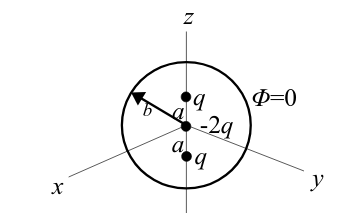
\includegraphics[width=8cm]{figure1}
\end{figure}

\begin{enumerate}[(a)] 
\item Escriba el potencial de las tres cargas en la ausencia de la esfera aterrizada. Encuentra la forma límite del potencial cuando $a \to 0$, mientras el producto $qa^2 = Q$ permaneces finito. Escriba esta última respuesta en coordenadas esféricas.

\item La presencia de la esfera aterrizada de radio $b$ altera el potencial para $r < b$. El potencial añadido puede ser visto como el causado por la densidad superficial de carga inducida en la superficie interna en $r = b$ o por cargas imagen localizadas en $ r > b$. Utilice la superposición para satisfacer las condiciones de frontera y encuentre el potencial en cualquier parte dentro de la esfera para $ r < a $ u $r > a$. Muestre que en el 
límite cuando $a \to 0$:
\begin{equation}
    \Phi(r,  \theta, \phi) \to \frac{Q}{2\pi \varepsilon_0 r^3} \left(1 - \frac{r^5}{b^5} \right) P_2 (\cos \theta)
\end{equation}
\end{enumerate}

\subsection*{Solución 3.7}

Partimos de la solución del potencial para una carga puntual. Añadimos potenciales para caca carga puntual, en este caso son 3 potenciales:
\begin{equation} 
\Phi(\mathbf{r}) = \frac{1}{4\pi\varepsilon_0} \frac{q}{|\mathbf{r} - a \mathbf{\hat{z}}|}  + \frac{1}{4\pi\varepsilon_0} \frac{q}{|\mathbf{r} - a (-\mathbf{\hat{z}})|} - \frac{2q}{4\pi\varepsilon_0}\frac{1}{|\mathbf{r}|}
\end{equation}

Para resolver este potencial utilizamos la expansión en serie de los polinomios de Legendre:


\begin{equation}
    \frac{1}{|\mathbf{r}- \mathbf{r_0}|} = \sum_{l=0}^{\infty} \frac{r_0^l}{r^{l+1}}P_{l}(\cos \theta) \quad \quad si \quad r > r_0
\end{equation}


\begin{equation}
    \frac{1}{|\mathbf{r}- \mathbf{r_0}|} = \sum_{l=0}^{\infty} \frac{r^l}{r_0^{l+1}}P_{l}(\cos \theta) \quad \quad si \quad r < r_0
\end{equation}


Para el caso del potencial propuesto, si $r>a$:
\begin{equation}
    \Phi(\mathbf{r}) = \frac{q}{4\pi\varepsilon_0} \sum_{l=0}^{\infty}\frac{a^l}{r^{l+1}}P_l(\cos \theta) + \frac{q}{4\pi \varepsilon_0}\sum_{l=0}^{\infty} \frac{(-1)^la^l}{r^{l+1}}P_l(\cos \theta) - \frac{2q}{4\pi\varepsilon_0}\frac{1}{r}
\end{equation}
Factorizamos el termino de la carga y las constantes:

\begin{equation}
    \Phi(\mathbf{r}) = \frac{q}{4\pi \varepsilon_0} \left [\sum_{l = 0}^{\infty} (1 + (-1)^l)\frac{a^l}{r^{l+1}}P_l (\cos\theta) - \frac{2}{r} \right]
\end{equation}


Ahora si $l = 1, 3, 5, ...$ los términos de la sumatoria se anulan y el potencial sólo depende del término de las dos cargas, si $l = 0$ también se anula la suma, pero si $l = 2, 4, 6,...$ entonces la suma toma la siguiente forma:


\begin{equation}
    \Phi(\mathbf{r}) = \frac{2q}{4\pi\varepsilon_0} \sum_{l = 2, 4, 6, ...}^{\infty} \frac{a^l}{r^{l+1}}P_l(\cos \theta)
\end{equation}


para el caso de $r < a$
\begin{equation}
    \Phi(\mathbf{r}) = \frac{2q}{4\pi\varepsilon_0} \sum_{l = 0}^{\infty} \frac{r^l}{a^{l+1}}P_l(\cos \theta) + \frac{2q}{4\pi\varepsilon_0} \sum_{l=0}^{\infty} (-1)^l \frac{r^l}{a^{l+1}}(-1l)^l \frac{r^l}{a^{l+1}} P_l(\cos \theta) - \frac{2q}{4\pi\varepsilon_0}\frac{1}{r}
\end{equation}

\begin{equation}
    \Phi(\mathbf{r}) = \frac{q}{4\pi \varepsilon_0} \left [\sum_{l = 0}^{\infty} (1 + (-1)^l)\frac{r^l}{a^{l+1}}P_l (\cos\theta) - \frac{2}{r} \right]
\end{equation}

En este caso cuando $l = 1, 3, 5, 7, ...$ la suma se desvanece
\begin{equation}
        \Phi(\mathbf{r})   = \frac{q}{4\pi\varepsilon_0} \left[ -\frac{1}{r} + \sum_{l = 0, 2, 4, ...}^{\infty}\frac{r^l}{a^{l+1}}P_l(\cos \theta) \right]
\end{equation}

Expandimos los dos primeros términos de las sumas:
$r < a$:
\begin{equation}
    \Phi(\mathbf{r}) = \left(\frac{2q}{4\pia\varepsilon_0} \right) \left[ \frac{a^2}{r^{3}}P_2(\cos \theta) + \frac{a^4}{r^5} P_4(\cos \theta) + ... \right ]
\end{equation}

Tomando $P_2(\cos\theta) = \frac{1}{2} (3\cos^2\theta - 1) $ definimos $Q = qa^2$ y cuando $a \to 0$ todos los términos de la suma del caso cuando $r < a$ se desvanecen, en cambio sólo sobreviven conservamos el primer término de la suma cuando $r > a$

\begin{equation}
    \Phi(\mathbf{r}) = \frac{2 Q }{4\pi \varepsilon_0} \frac{1}{2}(3 \cos^2 \theta -1 ) = \frac{Q}{4\pi\varepsilon_0} \frac{1}{r^3}(3\cos^2 \theta - 1)
\end{equation}

El término $l = 0$ corresponde a la carga total del sistema y debido que la carga está encerrada, la carga total es 0, el término $l = 1$ corresponde al término del momento dipolar y también se desvanece debido a la simetría de las cargas, así que el primer término diferente de cero es el término del momento cuadrupolar ($l= 2$)

\subsubsection*{(b)}
El problema añadiendo la esfera aterrizada de radio $b$ puede ser resuelto por el método de imágenes. En particular, la carga imagen genera el siguiente potencial:

\begin{equation} 
\Phi(\mathbf{r}) = \frac{1}{4\pi\varepsilon_0} \frac{q}{|\mathbf{r} - a \mathbf{\hat{z}}|}  +
\frac{1}{4\pi\varepsilon_0} \frac{q}{|\mathbf{r} - a (-\mathbf{\hat{z}})|} - \frac{2q}{4\pi\varepsilon_0}\frac{1}{|\mathbf{r}|} +  \frac{2q}{4\pi\varepsilon_0}\frac{1}{b} - \frac{1}{4\pi \varepsilon_0}\frac{q\frac{b}{a}}{|\mathbf{r} - (b^2/a)\mathbf{\hat{z}}|} - \frac{1}{4\pi \varepsilon_0}\frac{q\frac{b}{a}}{|\mathbf{r} + (b^2/a)\mathbf{\hat{z}}|}
\end{equation}

\begin{equation}
    \Phi(\mathbf{r}) = \frac{q}{4\pi\epsilon_0} \left [ -\frac{2}{r} + \frac{1}{|\mathbf{r} - a \mathbf{\hat{z}}|} + \frac{1}{|\mathbf{r} + a \mathbf{\hat{z}}|} + \frac{2}{b} - 
    \frac{b/a}{|\mathbf{r} - (b^2/a) \mathbf{\hat{z}}|} - \frac{b/a}{|\mathbf{r} + (b^2/a) \mathbf{\hat{z}}|}
    \right] 
\end{equation}
Utilizamos los polinomios de Legendre para cada término de las cargas en el potencial $\Phi(\mathbf{r})$ y consideramos $r > a$:
\begin{equation}
\begin{split}
    \Phi(\mathbf{r}) = \frac{q}{4\pi\varepsilon_0}
    \left (\sum_{l=0}^{\infty}\frac{a^l}{r^{l+1}}P_l(\cos \theta) -
    \frac{b}{a}\sum_{l=0}^{\infty}\frac{r^l}{(b^2/a)^{l+1}}P_l(\cos \theta) + \right .\\ 
    \left . \sum_{l=0}^{\infty} \frac{(-1)^l a^l}{r^{l+1}}P_l(\cos \theta) -\frac{b}{a}\sum_{l=0}^{\infty} \frac{(-1)^l r^l}{(b^2/a)^{l+1}}P_l(\cos \theta) - \frac{2}{r} + \frac{2}{b} \right)
\end{split}
\end{equation}

Agrupando los términos:
\begin{equation}
    \Phi(\mathbf{r}) = \frac{q}{4\pi\varepsilon_0} \left[ \frac{2}{b} - \frac{2}{r}+ \sum_{l=0}^{\infty} \left (\frac{a^l}{r^{l+1}} - \frac{b}{a}\frac{r^l}{(b^2/a)^{l+1}}  \right ) [P_l(\cos \theta) + P_l(\cos\theta)] \right]
\end{equation}
Tomando en cuenta que los términos impares de la suma desaparecen:

\begin{equation}
    \Phi(\mathbf{r}) = \frac{2q}{4\pi\varepsilon_0} \left[\frac{1}{b} - \frac{1}{r} + \sum_{l = 0, 2, 4, 6, ...}^{\infty} \left( \frac{a^l}{r^{l+1}} - \frac{1}{b}\left (\frac{ar}{b^2}\right )^l \right) P_l(\cos\theta)   \right]
\end{equation}
Cuando $l = 0$ los términos de la suma se anulan con $1/b$ y $1/r$
\begin{equation}
    \Phi(\mathbf{r}) = \frac{q}{2\pi\varepsilon_0} \sum_{l = 2, 4, 6, ...}^{\infty} \left( \frac{a^l}{r^{l+1}} - \left( \frac{1}{b}\frac{ar}{b^2}\right)^l \right)P_l(\cos\theta)
\end{equation}

\begin{equation}
    \Phi(\mathbf{r}) = \frac{q}{2\pi\varepsilon_0} \sum_{l = 2, 4, ...}^{\infty}\frac{a^l}{r^{l+1}}\left(1 - \left( \frac{r}{b}\right)^{2l+1} \right)P_l(\cos\theta)
\end{equation}

Como en el el inciso a) del problema, sólo consideramos el primer término de la suma cuando $a\to 0$:
\begin{equation}
    \Phi(\mathbf{r}) = \frac{q}{2\pi\varepsilon_0}\left[ \left(  \frac{a^2}{r^3}\left(1 - \left(\frac{r}{b} \right)^5 \right) \right )P_2(\cos\theta) + \left( \frac{a^4}{r^5} \left( 1 - \left(\frac{r}{b} \right )^{7} \right) \right)P_4(\cos\theta) + ... \right]
\end{equation}

Tomando $Q = qa^2$
\begin{equation}
    \Phi(\mathbf{r})=  \frac{Q}{2\pi\varepsilon_0 r^3} \left( 1 - \left( \frac{r}{b}\right)^5 \right)P_2(\cos\theta)   =
    \frac{Q}{2\pi\varepsilon_0 r^3} \left( 1 - \left( \frac{r}{b}\right)^5 \right)\frac{1}{2}(3\cos^2\theta -1)  
\end{equation}
\begin{equation}
    \Phi(\mathbf{r})=  \frac{Q}{4\pi\varepsilon_0 r^3} \left( 1 - \left( \frac{r}{b}\right)^5 \right)(3\cos^2\theta -1)
\end{equation}


\end{document}
